% =============================================================
%  Reading the Banished: A Deep-Learning Emotion Analysis of
%  Tang--Song Exiled Literati
%  -- English manuscript (single column, arXiv/CL readable)
%  Compile: xelatex tangsong_nlp_paper.tex   (ctex handles CJK)
%  Numbers traceable via recompute_all.py -> numbers_ledger.json
% =============================================================
\documentclass[10pt]{article}
\usepackage[UTF8]{ctex}
\usepackage{geometry}
\geometry{a4paper,margin=1in}
\setlength{\emergencystretch}{2em}
\usepackage{booktabs}
\usepackage{multirow}
\usepackage{array}
\usepackage{amsmath}
\usepackage{amssymb}
\usepackage{graphicx}
\usepackage{url}
\usepackage{xcolor}
\usepackage{float}
\usepackage{natbib}
\setlength{\bibsep}{0.5ex}
\bibliographystyle{plainnat}

% ctex localises float/reference names by default; force English for
% an English-language NLP manuscript (CJK glyphs still render fine).
\renewcommand{\figurename}{Figure}
\renewcommand{\tablename}{Table}
\renewcommand{\refname}{References}
\renewcommand{\abstractname}{Abstract}
\renewcommand{\appendixname}{Appendix}

\title{Reading the Banished: A Deep-Learning Emotion Analysis of
Tang--Song Exiled Literati}

\author{Shujiang Tang\\
Hunan University of Science and Engineering\\
\texttt{sjtang@huse.edu.cn}}
% For blind submission, replace the block above with:
% \author{Anonymous Authors\\ Anonymous Institution}

\date{}

\begin{document}
\maketitle

\begin{abstract}
The literature of political exile (\emph{bianzhe wenxue} 贬谪文学) is one of the
richest psychological archives in Chinese letters, yet its affective texture has
been characterised almost entirely through close reading. We build a reproducible
instrument for measuring it. A transparent five-dimensional \emph{emotion--imagery}
lexicon supplies the interpretable anchor, and a character-level CNN trained on that
lexicon predicts its scalar Affective Balance Index (ABI) directly from raw
characters (test $r{=}0.934$, Spearman $\rho{=}0.912$, MAE $6.26$). The correlation
measures agreement with the lexicon, the network's training target; affective
validity is inherited from the lexicon rather than established independently.
Applied to 21{,}287 Tang and Song \emph{shi} poems, the instrument yields comparable
profiles for twelve named banished officials: 韩愈 Han Yu and 秦观 Qin Guan are the
bleakest; 白居易 Bai Juyi, 黄庭坚 Huang Tingjian, 范仲淹 Fan Zhongyan and 辛弃疾 Xin
Qiji lie clearly on the easeful side; 柳宗元 Liu Zongyuan, 刘禹锡 Liu Yuxi, 苏轼 Su
Shi, 欧阳修 Ouyang Xiu and 王禹偁 Wang Yucheng are statistically indistinguishable
from neutral. Two checks bound these readings. Against two rounds of blind,
double-coded human gold standards, agreement is moderate (poem-level $\rho{=}0.46$,
author-level $r{=}0.57$)---an upper bound, since gold and instrument share a category
scheme. A transmission control finds two digitizations of one Tang work near-invariant
($A{=}0.960$), while two independently compiled Song anthologies raise imagery and
easeful vocabulary and leave a reproducible dimension-level editorial signature; the
net scalar is unchanged for the imperial anthology and shifts for the private one. A
within-author dose--response over 苏轼 finds no net exile effect, only a single dark
stretch at 黄州---a directional observation offered alongside the exile-gloom
scholarship, not against it. Per-poem prediction RMSE ($8.97$) is roughly $4.6\times$
the inter-author dispersion (sd $1.93$), so the high correlation is earned on a scale
wider than the conclusions.
\end{abstract}

\section{Introduction}
\label{sec:intro}
The literature of political exile (\emph{bianzhe wenxue} 贬谪文学) forms one of the
most sustained psychological archives in Chinese letters. From 柳宗元 Liu Zongyuan
and 刘禹锡 Liu Yuxi in the Mid-Tang to 苏轼 Su Shi and 黄庭坚 Huang Tingjian in the
Song, poets demoted to frontier posts turned confinement into some of the period's
most introspective verse. Literary scholarship has long characterised these authors
through close reading \citep{shang2007exiled,xing2024liusu}. The aim of this paper is
to \emph{quantify} that scholarship, not to overturn it: we supply a reproducible,
auditable measurement of the exilic emotional register and set it against the
received literary findings as a complement to close reading. What has been missing
is a measurement that lets a reader compare such claims against the \emph{full corpus}
rather than a curated few, and that can be applied consistently across a cohort of
exiled officials.

Deep learning makes that measurement possible. Character-level convolutional
networks model style and sentiment directly from surface form
\citep{kim2014convolutional}, and classical-Chinese NLP has reached the point where
a poem's affective profile can be predicted from its characters alone
\citep{hou2015sentiment,du2025multimodal}. We exploit this to study the emotional
lives of exiled officials at scale. Our analyser is a CNN trained to predict a
transparent five-dimension \emph{emotion--imagery} lexicon: two poles
(sorrow--loneliness and detached--easeful) plus a scalar summary. The network
recovers only the two emotional poles well (sorrow--loneliness Pearson
$r{=}0.86$, detached--easeful $r{=}0.85$), while the three middle dimensions stay
near zero (exile--journey $r{=}0.05$, nature--landscape $r{=}0.15$,
void--temporality $r{=}0.07$); it recovers the interpretable lexicon that motivates
it and, because it reads raw characters, demonstrates that the part of the affect
signal the lexicon can measure is present in surface form rather than in our
counting choices. The network's role should be stated up front: it is the
\emph{carrier} of the signal, not its source---its validity is inherited from the
transparent lexicon it was trained on, and its high recovery rate is not independent
validity evidence (\S\ref{sec:dl}).

One threat must be controlled before any poet score can be trusted. Classical
poems reach us through two very different kinds of channel. The first is
\emph{reprinting}: the same work, re-edited across centuries, survives in two or
more digitized witnesses whose variants are local---a graph here, a line there. The
second is \emph{selection}: an anthology chooses a subset of a poet's corpus
according to an explicit aesthetic programme, which may systematically prefer one
register over another. A word-frequency affect measure is near-invariant under the
first and can be re-weighted under the second. Prior affect studies report a poet's
score from a \emph{single} edition and read it as a property of the poet, hiding
the assumption that the number is a property of the author rather than of the
particular text that happened to survive. We therefore treat cross-edition
agreement not as the paper's subject but as a \emph{robustness control}: if the
emotion signal we recovered survives both regimes of transmission, it is a property
of the poets, not of their editions.

\paragraph{Contributions.} Prior affect work reports a poet's score from a single
edition and reads it as a property of the author
\citep{hou2015sentiment,du2025multimodal}. This paper makes three claims that depart
from that practice.
\begin{itemize}
\item \textbf{A transparent affect instrument with a measured validation envelope.} A
hand-built five-dimension emotion--imagery lexicon, summarised by the ABI, is checked
against two rounds of blind double-coding (450 poems; 40 authors with $\ge5$ gold
poems each). Coding reliability replicates ($\kappa_w$ $0.82$--$0.91$, ordinal
$\alpha$ $0.95$--$0.97$); poem-level criterion agreement is $\rho{=}0.46$
$[0.39,0.53]$ and author-level agreement within the short-poem gold subsample
(20--160 characters) is $r{=}0.57$ $[0.36,0.73]$, rising to $0.79$ for the cohort.
The $r{=}0.57$ bounds the lexicon's agreement with human coding \emph{within that
subsample}; it does not validate the full-collection values in Table~\ref{tab:abi},
and for five of the eight target authors with subsample means the two signs differ,
because short poems carry fewer scenery words. A character-level CNN delivers the
same index from raw characters (test $r{=}0.934$) but never significantly beats the
lexicon it distils---the lexicon, not the network, is the measuring device.

\item \textbf{Emotional profiles of twelve exiled officials.} Ranked on the
desolate--easeful axis (Table~\ref{tab:abi}), 韩愈 and 秦观 are the only two figures
clearly below zero; 白居易, 黄庭坚, 范仲淹 and 辛弃疾 lie clearly above it; 刘禹锡,
苏轼, 欧阳修, 柳宗元 and 王禹偁 are indistinguishable from neutral, with 陆游 weakly
easeful. The near-neutral 柳宗元 departs from 尚永亮's portrait, whose core evidence
lies outside the \emph{shi} layer, while 刘禹锡's neutrality is compatible with his
``poet-hero'' epithet.

\item \textbf{Transmission robustness and the analyses it licenses.} We check the
signal against its two transmission regimes---reprinting and independent
selection---and find a reproducible dimension-level editorial signature but no
uniform stability of the net index (\S\ref{sec:robust}); the dimension-level signal
is therefore not a version artefact. Two analyses follow. A counterfactual projection
attributes a measured profile to its survival channels. A within-author dose--response
over 苏轼 finds no net exile effect ($-0.56$ $[-2.37,+1.25]$) but a raised lexical
gradient with severity ($+3.07$ per grade)---three periods, and directional evidence
only.
\end{itemize}

\section{Related Work}
\label{sec:related}
\paragraph{Close reading of exile.} Within literary studies, the emotional world of the
banished official has been mapped by close reading: 尚永亮 \citep{shang2007exiled}
reads the Yuanhe exiles as dominated by anxiety and a sense of abandonment, and
邢若琳 \citep{xing2024liusu} contrasts the ``angry, solitary'' 柳宗元 with the
``detached, easeful'' 苏轼. Such readings are interpretively rich but rest on curated
selections of verses: they cannot test whether a claim about one poet's posture holds
across his full surviving corpus, and they yield no instrument that a second scholar
could rerun. Supplying that instrument---and checking its readings against the
close-reading tradition---is the purpose of \S\ref{sec:profiles}.

\paragraph{Sentiment analysis for classical Chinese poetry.} On the computational
side, affect prediction from classical verse began with lexicon- and rule-based
studies \citep{hou2015sentiment} and has moved to neural representations:
\citet{du2025multimodal} combine textual, pictorial and recitation signals for poetry
sentiment classification, and \citet{fang2011cld} analyse imagery-based style in Song
\emph{ci}; recent work continues along this line: \citet{liu2025samcap} fuse textual
and knowledge-base features through multi-dimensional attention for classical-poetry
sentiment analysis, and \citet{qin2025shades} quantify eighteen aesthetic moods of
classical Chinese poetry with NLP-based empirical methods and release them as a
searchable database. These systems evaluate poem-level classification on modern
anthologies, take the anthology text as given, and report affect from a single
edition; none validates the affect measure against blind human coding, and none asks
whether the signal survives transmission. We differ on all three counts: author-level
measurement over complete collections, validation on a blind double-coded gold set
(\S\ref{sec:gold}), and a transmission-robustness control (\S\ref{sec:robust}).

\paragraph{Computational stylometry and authorship attribution.} Authorship
identification for Tang poetry is an active task \citep{shiziren2022,zhou2021lda},
extending the broader stylometric tradition \citep{stamatatos2009survey};
quantitative analysis has also been applied to canon formation
\citep{wang2008finding} and to an individual exile's self-presentation
\citep{wang2023lideyu}. Attribution asks who wrote a text and is validated against
known authorship; affect measurement enjoys no such ground truth, so our validation
rests instead on a human gold standard and on cross-edition concordance rather than
on classification accuracy.

\paragraph{Digital philology of transmission.} The variants introduced by centuries
of recension are themselves an object of computational study \citep{yuan2023variants},
and digital-humanities work has mapped the spatio-temporal trajectories of the
\emph{Quan Tang Shi} exiles \citep{bianzhe2022}. Philology treats such variants as
objects of study in their own right; we treat edition provenance as a
measurement-theoretic threat---an affect score computed from one edition may be an
artefact of that edition---and build the control that quantifies it.

\section{Method}
\label{sec:method}
\subsection{Task and data}
\label{sec:data}
\paragraph{Task formulation.} Given a poem as a raw character sequence, the
analyser predicts a five-dimension \emph{emotion--imagery} profile
$\phi\in\mathbb{R}_{\ge0}^{5}$---悲苦孤寂 sorrow, 贬谪羁旅 exile--journey, 旷达闲适
easeful, 自然山水 nature--landscape, 空幻时空 void--temporality, each a rate per
1{,}000 characters---together with its scalar summary, the ABI (Affective Balance Index)
$\mathrm{ABI}{=}\phi_{\textsc{Kuang}}{-}\phi_{\textsc{Bei}}$ (rates are already per 1{,}000 characters). Author-level
scores aggregate poem-level predictions over one author's poems; every claim in
this paper is made at the author or corpus level, never for a single poem. The
model is trained against a transparent lexicon (\S\ref{sec:lexicon}) and evaluated
on three criteria: agreement with the lexicon target (\S\ref{sec:dl}), consistency
with a blind double-coded human gold set (\S\ref{sec:gold}), and cross-edition
concordance of author-level scores (\S\ref{sec:robust}).

\subsubsection{The exiled-literati cohort}
\label{sec:cohort}
We read ``exiled'' (\emph{bianzhe}) as a spectrum rather than a single paradigm. The
core cohort are classical \emph{zhuchen} 逐臣---officials formally banished to remote
posts: 柳宗元, 刘禹锡, 韩愈 and 白居易 in the Tang; 王禹偁, 范仲淹 and 欧阳修 in the
Song. A second tier broadens the term to repeated demotion or political
marginalisation: 苏轼, 黄庭坚 and 秦观; 陆游's serial dismissal and frontier posting
place him here even without the classical 逐臣 pattern, and 辛弃疾---primarily a
\emph{ci} 词 poet who spent decades in political retirement---is included as the
marginal ``non-classical'' case. All twelve are named and justified; none is included
silently. These twelve are the \emph{subjects} of the emotion analysis in
\S\ref{sec:profiles}; their exile chronologies are given in the
Supplementary Material (App.~C).

\subsubsection{Text corpora}
\label{sec:corpus}
Primary editions are \emph{Quan Tang Shi} (全唐诗, QTS) and \emph{Quan Song Shi}
(全宋诗, QSS), the standard complete collections in the Book1Q84 / Chinese Textware
corpora. We build a unified poetry layer of 21{,}287 Tang and Song \emph{shi} poems,
eliminating genre mixing that would confound affect, and add 1{,}854 Tang prose texts
(686{,}766 characters) used only for a side probe (Supplementary Material, App.~A).

For the transmission-robustness control of \S\ref{sec:robust} we draw on two further
digitizations. On the Tang side, \emph{Yu Ding Quan Tang Shi} (御定全唐詩, YD) is the
Kangxi-era imperially commissioned collection of which the modern QTS is a re-edited
reproduction, so the two are \emph{two digitizations of one work} (we obtained 899 of
900 \emph{juan}). On the Song side we use two independent selection anthologies, one
imperial and one private: \emph{Yu Xuan Song Shi} (御選宋詩), the Song portion of the
Kangxi anthology \emph{Yu Xuan Song Jin Yuan Ming Si Chao Shi} (kanripo KR4h0143
\citealp{kangxi1709}), and \emph{Song Shi Chao} (宋詩鈔, kanripo KR4h0157,
\citealp{wu1671}). The imperial anthology parses to 9{,}405 poems by 660 authors, the
private one to 9{,}612 poems by 76 authors over 829{,}341 characters of verse (Supplementary Material, App.~A). Both belong to the same \emph{Siku Quanshu} Wenyuange
base-edition family and pass through the same pipeline, so any difference between them
is attributable to selection principle rather than to edition, orthography or parsing.

\subsection{A transparent emotion--imagery lexicon (interpretable anchor)}
\label{sec:lexicon}
We define five transparent categories $\mathcal{C}{=}\{C_1,\dots,C_5\}$. Two are
\emph{affective poles} whose valence contrast defines the scalar index:
\textbf{悲苦孤寂} (sorrow--loneliness, \textsc{Bei}) and \textbf{旷达闲适}
(detached--easeful, \textsc{Kuang}). One is a \emph{thematic} category denoting the
named condition of exile rather than a felt affect: \textbf{贬谪羁旅} (exile--journey,
\textsc{Bian}). Two are \emph{imagistic registers} of banishment verse rather than
emotions proper: \textbf{自然山水} (nature--landscape, \textsc{Zi}) and
\textbf{空幻时空} (void--temporality, \textsc{Kong}). A hand-curated lexicon
$\mathcal{L}$ partitions words into the five categories. For author $a$ with
character count $N_a$ and text $T_a$,
\begin{equation}
\phi_{a,k} = \frac{\sum_{w\in\mathcal{L}_k}\mathrm{count}(w,T_a)}
                   {N_a}\times 1000,
\qquad k\in\mathcal{C}.
\end{equation}
The \textbf{ABI} contrasts the two \emph{affective} poles:
\begin{equation}
\mathrm{ABI}(a)=\phi_{a,\textsc{Kuang}}-\phi_{a,\textsc{Bei}}.
\end{equation}
Every value is thus a verifiable function of word counts; no parameter is learned.
We stress what ABI is and is not: it is the signed difference of two word rates,
not a calibrated psychological scale. Its validity as an \emph{affect} index rests
on the two poles being valence-opposed; the other three dimensions are read
separately and are not folded into the scalar.

\subsection{The deep-learning analyser}
\label{sec:dl}
M1 is the hand-curated lexicon counting layer, the interpretable layer that reports
the twelve rankings. The measurement itself is delivered by a character-level CNN
trained to regress the lexicon's five-dimension profile and its scalar ABI from raw
poem characters. It recovers the anchor well (test Pearson $r{=}0.934$, Spearman
$\rho{=}0.912$, MAE $6.26$; pool $n{=}20{,}912$, the unified layer minus 375
three-sigma ABI outliers) but unevenly across dimensions: the two emotional poles are
reproduced (sorrow--loneliness $r{=}0.86$, detached--easeful $r{=}0.85$) while the
three middle dimensions stay near zero (exile--journey $0.05$, nature--landscape
$0.15$, void--temporality $0.07$). This $r$ measures agreement with the lexicon, the
network's training target, so the analyser's \emph{affect} validity is inherited from
the lexicon rather than established independently, and the lexicon's own agreement
with blind human coding is only moderate ($\rho{=}0.46$, \S\ref{sec:gold}). The
decisive point is that the network reads \emph{raw characters}: the affect signal it
predicts is present in surface form, not an artefact of how we count words.
Architecture and hyperparameters are given in the reproduction package
(\S\ref{sec:repro}).

Three variants test whether the signal rests on the counting scheme or on surface form
(Table~\ref{tab:agree}). An IDF-weighted lexicon (M2) tracks the base lexicon closely
($r{=}0.994$, $\rho{=}0.97$), so the index is insensitive to the weighting scheme. A
geometry-only LSA estimator (M3), character $n$-gram TF-IDF with TruncatedSVD and
seed-phrase centroids, never sees the counting lexicon and correlates with it at only
$r{=}0.31$---about a third of the network's. An LDA estimator (M4) assigns zero
valence to every topic, whose top tokens lie outside both poles, and yields zero
variance. The M3/M4 failure is informative: unsupervised geometry captures little of
the affect axis, most plausibly reflecting authorial and period style, which is what
justifies a \emph{transparent, hand-specified lexicon} as the anchor and what the
supervised CNN succeeds in recovering.

\begin{table}[H]
\centering\footnotesize
\caption{Agreement of variant estimators with the lexicon-based profile (Pearson
$r$ / Spearman $\rho$).}
\label{tab:agree}
\begin{tabular}{lcc}
\toprule
Estimator & $r$ & $\rho$\\
\midrule
M2 IDF-weighted lexicon & $0.994$ & $0.972$\\
M3 LSA geometric & $0.308$ & $0.112$\\
M4 LDA topics & \multicolumn{2}{c}{undefined (zero variance)}\\
\bottomrule
\end{tabular}
\end{table}

\subsection{Analyser selection}
\label{sec:extbench}

To fix the analyser, we position it against recent strong convolutional and hybrid
architectures under one shared protocol: the same 20{,}912-poem pool, a 5-fold
partition with per-poem out-of-fold prediction (so no poem is scored by a model that
saw it in training), 14 epochs, and a fixed seed. The baselines are 1D sequence
adaptations of vision CNNs published in 2025--2026: OverLoCK \citep{overlock2025},
TransXNet \citep{transxnet2025}, PFGNet \citep{pfgn2026}, TACNN \citep{tacnn2026} and
FA-CNN \citep{facnn2026}; our entry is the proposed AttentionFractal CNN, a
character-level fractal convolutional network whose multi-head readout produces a
per-character saliency map.

\begin{table}[H]
\centering\footnotesize
\caption{Extended benchmark: poem-level ABI regression under a shared protocol
(identical 20,912-poem pool, 5-fold CV with per-poem out-of-fold prediction, 14
epochs, seed 20260918). CV $r$ is mean$\pm$std across folds; author-level
$\rho$ is Spearman between model-predicted and lexicon ABI across the 12 named
officials; gold $\rho$ is Spearman between model prediction and the two-coder
human double-coding consensus on the 160-poem double-coded set (lexicon baseline shown for
reference). The last three rows of the proposed family are structural variants of
the AttentionFractal CNN (deep bottleneck, lexicon-feature channel, attention
consistency).}
\label{tab:extbench}
\begin{tabular}{lccccc}
\toprule
Model & Params (M) & CV $r$ & Author $\rho$ & Gold $\rho$ (ours) & Gold $\rho$ (lexicon)\\
\midrule
\multicolumn{6}{l}{\emph{Baselines (1D adaptations of 2025/2026 vision CNNs)}}\\
Wide plain CNN & 0.60 & $0.9737{\pm}0.0021$ & 0.993 & 0.403 & 0.419\\
OverLoCK-1D \citep{overlock2025} & 0.90 & $0.9685{\pm}0.0027$ & 1.000 & 0.418 & 0.419\\
TransXNet-1D \citep{transxnet2025} & 0.64 & $0.9801{\pm}0.0020$ & 0.993 & 0.411 & 0.419\\
PFGNet-1D \citep{pfgn2026} & 0.74 & $0.9696{\pm}0.0026$ & 1.000 & 0.457 & 0.419\\
TACNN-1D \citep{tacnn2026} & 0.58 & $0.9733{\pm}0.0013$ & 0.993 & 0.427 & 0.419\\
FA-CNN-1D \citep{facnn2026} & 0.68 & $0.9743{\pm}0.0012$ & 0.993 & 0.437 & 0.419\\
\multicolumn{6}{l}{\emph{Proposed: AttentionFractal CNN}}\\
AttentionFractal-CNN (proposed) & 0.63 & $0.9840{\pm}0.0018$ & 1.000 & 0.407 & 0.419\\
\quad + deep bottleneck & 0.65 & $0.9864{\pm}0.0027$ & 1.000 & 0.431 & 0.419\\
\quad + lexicon-feature channel & 0.63 & $0.9891{\pm}0.0019$ & 0.993 & 0.426 & 0.419\\
\quad + attention consistency & 0.63 & $0.9878{\pm}0.0012$ & 1.000 & 0.431 & 0.419\\
\multicolumn{6}{l}{\emph{Ablation: pure Transformer (no convolution)}}\\
Transformer-1D (no conv.\ inductive bias) & 1.55 & $0.9850{\pm}0.0028$ & 0.993 & 0.416 & 0.419\\
\bottomrule
\end{tabular}
\end{table}

Table~\ref{tab:extbench} reports poem-level ABI regression. Every architecture
converges to a narrow band ($r\approx0.969$--$0.989$), within fold-to-fold noise: at
the poem level the gap between architectures is far smaller than their distance to
the noise floor, and even a pure Transformer without convolutional bias matches the
convolutional family ($0.9850$). Per-poem precision therefore does not select the
analyser. Three properties do: the multi-head readout yields a per-character saliency
map that can be aligned with the lexicon mask; every model reproduces the ordering of
the twelve officials (author-level Spearman $0.99$--$1.00$, Table~\ref{tab:abi}); and
on the 160-poem double-coded set, model predictions correlate with the human
consensus at $\rho\approx0.40$--$0.46$, level with the lexicon baseline of $0.419$ and
none significantly above it. We present a SOTA-comparable, interpretable instrument,
not one with superior per-poem precision; these out-of-fold estimates are tighter
than the single-split $r{=}0.934$ of \S\ref{sec:dl} because they use the full pool and
a leakage-free partition.

\section{Experiments}
\label{sec:profiles}

\subsection{Validity against blind human coding}
\label{sec:gold}

Construct transparency is not validity. To test whether the profile measures anything
a reader of classical poetry would recognise as affect, we drew a stratified blind
sample of 160 \emph{shi} poems (80 Tang, 80 Song; 78 authors; 20--160 characters;
strata crossing dynasty, cohort membership and the lexicon's own ABI median) and had
two domain experts---one working on Tang verse, one on Song---independently rate every
poem on the five categories, on a 0--3 ordinal scale, with author, title, dynasty and
all lexicon output hidden. The gold ABI is the coder-mean difference of the two
\emph{affective} poles, defined exactly as in Eq.~(2).

The coding is reliable. Quadratic-weighted $\kappa$ runs $0.72$--$0.88$ across the
five dimensions, ordinal Krippendorff $\alpha$ $0.93$--$0.97$, and the coders' gold
ABI values correlate at $r{=}0.90$ (ICC$(2,1){=}0.86$). A second independent sample
(292 poems, 42 authors) replicates this ($\kappa_w$ $0.82$--$0.91$, $\alpha$
$0.95$--$0.97$, $r{=}0.89$), with no drift in the standard. Because the raters applied
the instrument's own five-category scheme, their agreement partly reflects shared
category definitions, so the concurrently measured validity is a ceiling rather than
a lower bound.

The analyser's agreement with that judgement is moderate:
$\rho(\mathrm{ABI},\mathrm{ABI}_{\mathrm{gold}}){=}0.43$ $[0.26,0.55]$ on the first
sample, $0.46$ on the second, and $0.46$ $[0.39,0.53]$ pooled across both (450
poems), every interval excluding zero. With at least five gold poems per author (40
annotated authors qualify), the pooled author-level criterion is $r{=}0.57$
$[0.36,0.73]$, and the twelve cohort officials alone give $0.79$. This $r{=}0.57$
validates agreement only \emph{within} the short-poem gold subsample, not the
full-collection values of Table~\ref{tab:abi}: of the 12 target authors, 8 have
subsample means and 5 show full-collection signs \emph{opposite} them, because short
绝句 carry fewer scenic words and so a systematically lower normalised ABI. The
criterion is stable under dropping short, long or outlier poems ($0.43$--$0.46$) and
does not differ by source (collection $0.46$, anthology $0.43$). Two further checks
bound it: an out-of-author ridge fit from the five lexicon rates to gold ABI gives
$r{=}0.40$, $\rho{=}0.44$, indistinguishable from the within-sample criterion, and the
agreement holds for authors the model trained on ($\rho{=}0.48$) and for authors
absent from training ($0.38$), so it is not an author-leakage artefact.

The dimensions differ sharply in how well they are captured
(Table~\ref{tab:gold}): nature--landscape is tracked best ($\rho{=}0.54$),
sorrow--loneliness next ($0.45$), then exile--journey ($0.39$), with void--temporality
($0.30$) and easeful ($0.29$) weakest---a warning that the easeful pole, which defines
half the scalar, is the least well measured.

Two perturbation checks bound the lexicon. A leave-$k$-out test on four polysemous
easeful characters (醉, 啸, 傲, 狂; $17.2\%$ of easeful hits) preserves author
ordering ($\rho{=}0.97$) but shifts every ABI downward: their ``ease'' rests on
drinking and unrestrained-spirit \emph{subject matter}, not mood words. Per-author
sign-flip rates under $B{=}2{,}000$ draws removing a random $10\%$ of each pole's
entries (Table~\ref{tab:abi}) then separate the twelve placements: 韩愈 ($0.6\%$),
秦观 ($2.5\%$), 范仲淹 ($0.2\%$), 辛弃疾 ($0.1\%$), 黄庭坚 ($6.5\%$) and 白居易
($9.6\%$) hold their signs, while the six near-zero placements do not---欧阳修 is a
coin toss ($52.4\%$) and 柳宗元, 苏轼, 陆游, 刘禹锡 and 王禹偁 flip in $21$--$34\%$ of
draws. We adopt $20\%$ as a pre-defined conditional cut, sitting between the most
stable and the most unstable authors; placements above it are read as conditional on
the full lexicon throughout. Because 空幻时空 does not enter the scalar ABI, adding or
removing its entries cannot change that scalar, so its $\rho{=}1.00$ is definitional
rather than robustness evidence.

The analyser's defensible claim is ordinal, not scalar. Sorting the gold poems into
lexicon-ABI quintiles yields gold ABI means $-1.34$, $-0.59$, $-0.30$, $-0.02$,
$+0.55$, a monotonic ladder with top--bottom gap $+1.89$ $[+1.00,+2.63]$ and
$\rho{=}1.00$ across quintiles (Figure~\ref{fig:quintile}). The
analyser orders poems correctly in groups, and every ABI statement in this paper is an
author- or corpus-level claim, never a single-poem one.

\begin{table}[H]
\centering\footnotesize
\caption{Concurrent validity against a blind two-coder gold sample (160 poems, 78
authors). $\kappa_w$ = quadratic-weighted Cohen's $\kappa$; $\alpha$ = ordinal
Krippendorff's $\alpha$; $\rho$ = Spearman correlation of the per-poem ABI (lexicon-count
layer, the same source as the CNN)
with the coder-mean gold rating, cluster-bootstrapped over authors (95\% CI in
brackets). The composite row uses the two poles that define the index.}
\label{tab:gold}
\begin{tabular}{lcccc}
\toprule
Dimension & $\kappa_w$ & $\alpha$ & $\rho$ & 95\% CI\\
\midrule
悲苦孤寂 sorrow & $0.81$ & $0.96$ & $0.45$ & $[0.28,\,0.56]$\\
贬谪羁旅 exile & $0.88$ & $0.96$ & $0.39$ & $[0.24,\,0.53]$\\
旷达闲适 easeful & $0.77$ & $0.94$ & $0.29$ & $[0.15,\,0.42]$\\
自然山水 nature & $0.72$ & $0.93$ & $0.54$ & $[0.41,\,0.64]$\\
空幻时空 void & $0.75$ & $0.94$ & $0.30$ & $[0.16,\,0.46]$\\
\midrule
\multicolumn{5}{l}{\emph{Composite: ABI (coder agreement
ICC${=}0.86$, $r{=}0.90$)}}\\
ABI & --- & --- & $0.43$ & $[0.26,\,0.55]$\\
\bottomrule
\end{tabular}
\end{table}
\begin{figure}[t]
\centering
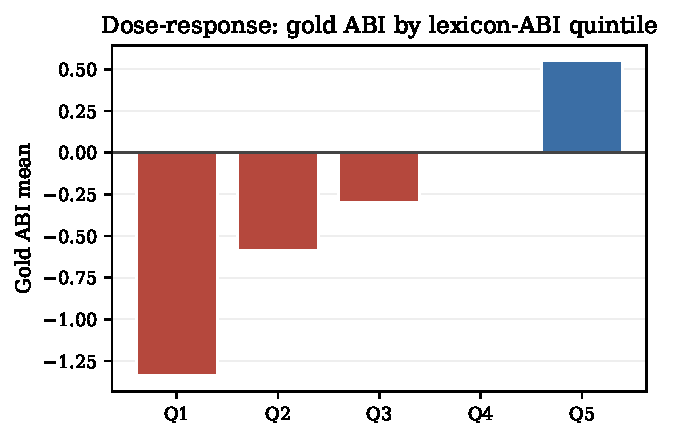
\includegraphics[width=0.60\linewidth]{figures/fig_quintile.pdf}
\caption{Gold ABI rises monotonically across lexicon-ABI quintiles (top$-$bottom $+1.89$ $[+1.00,+2.63]$); the analyser orders poems correctly ($\rho{=}1.00$ across quintiles).}
\label{fig:quintile}
\end{figure}
\subsection{Per-poet emotional profiles}
\label{sec:profiles:poets}
Table~\ref{tab:abi} reports the ABI for the twelve target authors with bootstrap 95\% CIs (B$=2{,}000$); Figure~\ref{fig:abi_authors} shows the bars in ascending bleak$\to$easeful order. 韩愈 ($-2.49$) and 秦观 ($-2.11$) are the only two placements clearly below zero, while 白居易 ($+1.76$), 黄庭坚 ($+1.34$), 范仲淹 ($+3.35$) and 辛弃疾 ($+4.25$) lie clearly above, 辛弃疾 and 范仲淹 the highest on the easeful side; 刘禹锡 ($-0.88$), 苏轼 ($+0.41$), 欧阳修 ($-0.18$), 柳宗元 ($+0.22$), 王禹偁 ($-0.98$) and 陆游 ($+0.57$, flip $26.8\%$) include zero and are statistically indistinguishable from neutral, so near-zero estimates are fragile (a fragility that resurfaces in \S\ref{sec:gold} and \S\ref{sec:robust}).

\begin{table}[H]
\centering\footnotesize
\caption{ABI (M1) by author, per 1{,}000 characters, with bootstrap
95\% CI over the complete-collection poems (B$=2{,}000$; negative = bleaker).
Intervals marked $^*$ include zero. \emph{Flip} (\%) is the sign-flip
probability: in each of $B{=}2{,}000$ draws a random $10\%$ of the entries in
each affective pole is removed and the author's ABI is recomputed from the
surviving word counts; \emph{flip} is defined as a sign reversal relative to the
unperturbed baseline under this lexicon perturbation, and it measures how strongly a
placement depends on the exact lexicon composition (a composition/sensitivity check),
not how valid the placement is. We adopt 20\% as a pre-defined conditional cut: it is
roughly the empirical upper bound on sign flips permitted by the sample size, and it
sits between the most-stable and the most-unstable authors; it does \emph{not} endorse
the $r{=}0.57$ validity claim. This table reports the interpretable M1 layer;
Table~\ref{tab:extbench} shows every model recovers the author-level ordering at
$\rho{=}0.99$--$1.00$, so this table's hierarchy invariance holds.}
\label{tab:abi}
\begin{tabular}{lrrr}
\toprule
Author & ABI & 95\% CI & Flip\\
\midrule
柳宗元 Liu Zongyuan & $+0.221$ & $[-2.12,\;2.68]^*$ & $34.2$\\
刘禹锡 Liu Yuxi & $-0.881$ & $[-2.38,\;0.59]^*$ & $26.9$\\
韩愈 Han Yu & $-2.491$ & $[-3.79,\;-1.29]$ & $0.6$\\
白居易 Bai Juyi & $+1.762$ & $[0.90,\;2.63]$ & $9.6$\\
苏轼 Su Shi & $+0.407$ & $[-0.36,\;1.14]^*$ & $28.2$\\
欧阳修 Ouyang Xiu & $-0.175$ & $[-1.35,\;1.08]^*$ & $52.4$\\
黄庭坚 Huang Tingjian & $+1.344$ & $[0.55,\;2.13]$ & $6.5$\\
秦观 Qin Guan & $-2.113$ & $[-4.03,\;-0.18]$ & $2.5$\\
王禹偁 Wang Yucheng & $-0.982$ & $[-2.36,\;0.29]^*$ & $21.1$\\
范仲淹 Fan Zhongyan & $+3.354$ & $[1.27,\;5.57]$ & $0.2$\\
辛弃疾 Xin Qiji & $+4.250$ & $[0.84,\;7.69]$ & $0.1$\\
陆游 Lu You & $+0.565$ & $[0.02,\;1.14]$ & $26.8$\\
\bottomrule
\end{tabular}
\end{table}

\begin{figure}[t]
\centering
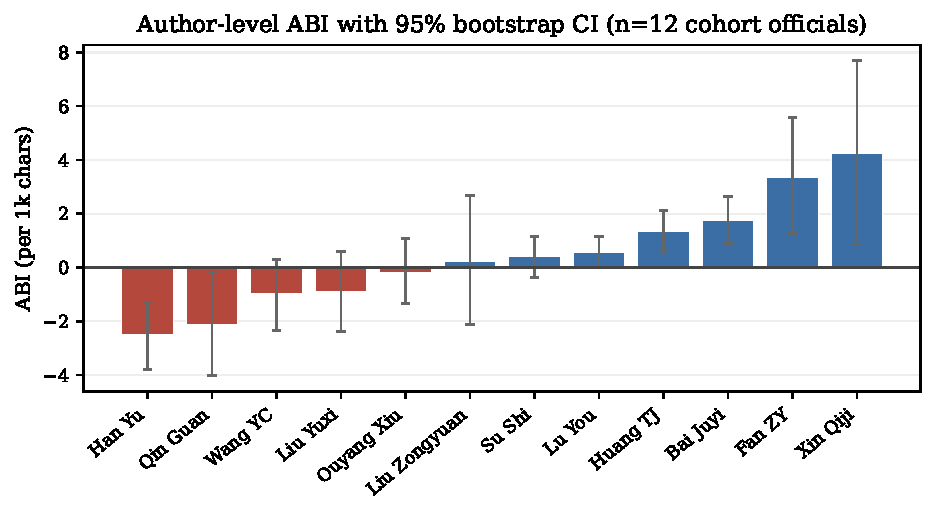
\includegraphics[width=0.62\linewidth]{figures/fig_abi_authors.pdf}
\caption{Author-level ABI (per 1k chars) with 95\% bootstrap CI. Han Yu and Qin Guan are the only two clearly below zero; six placements include zero (intervals marked $*$).}
\label{fig:abi_authors}
\end{figure}


\subsection{Affective versus imagistic dimensions}
\label{sec:profiles:dims}
The scalar ABI contrasts only the two affective poles; the three remaining dimensions are read separately and are where the exilic experience is most distinctly visible. 贬谪羁旅 (exile--journey) fires on 31.6\% of the unified \emph{shi} corpus, and the imagistic registers 自然山水 (nature--landscape, 77.4\%) and 空幻时空 (void--temporality, 62.5\%) dominate the exilic poem's scenery and temporal reflection (Figure~\ref{fig:dim_coverage}). As the transmission-robustness control (\S\ref{sec:robust}) shows, an editor's hand shows up precisely in these imagistic registers while the affective balance can stay near flat---the analyser must read both the scalar mood and the imagistic texture that shapes it.

\begin{figure}[t]
\centering
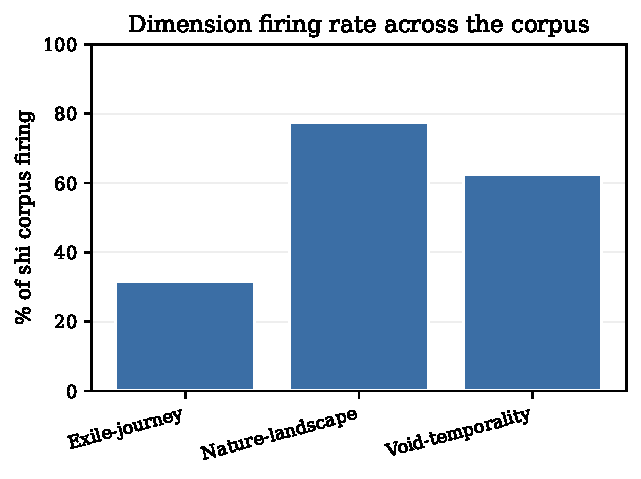
\includegraphics[width=0.60\linewidth]{figures/fig_dim_coverage.pdf}
\caption{Dimension firing rates across the corpus: exile--journey 31.6\%, nature--landscape 77.4\%, void--temporality 62.5\%.}
\label{fig:dim_coverage}
\end{figure}


\subsection{Alignment with scholarship}
\label{sec:profiles:lit}
Table~\ref{tab:lit} situates the twelve authors' ABI estimates against established
literary scholarship. At the author level 韩愈 is the bleakest and 陆游 sits just above
zero on the easeful side, placements that rest on a lexicon whose agreement with blind
human coding is moderate ($\rho{=}0.46$ pooled across the two rounds). The cohort-level
ranking is partially consistent with the received view that the Yuanhe exiles are
melancholic, and two cases deserve comment. 柳宗元's near-neutral index ($+0.22$)
diverges from 尚永亮's portrait of him as the bleakest Yuanhe exile; 尚's core evidence
lives in letters and \emph{fu} (e.g.\ 《寄许京兆孟容书》), not in the \emph{shi} layer,
and 柳's signature strategy is to displace grief into landscape and temporality---imagery
the lexicon reads as scenery, not sorrow---so the surface form structurally
underestimates such poets. 刘禹锡's near-neutral, slightly bleak value ($-0.88$,
interval including zero) does \emph{not} contradict Bai Juyi's epithet ``poet-hero''
(诗豪). The divergences therefore locate the instrument's limits rather than revise the
received view. Two caveats bound the reading further: 陆游's $+0.57$ exposes a construct
blind spot, since his corpus is $\approx$9{,}300 \emph{shi} poems against only
$\approx$140 \emph{ci} and the instrument does not measure loyalist grief; and the five
categories do not separately score 忧国忧民/忠愤 or 思乡, registers scholarship treats as
distinct, so the scalar ABI is a partial view of the exilic psyche.

\begin{table}[H]
\centering\footnotesize
\caption{Alignment with prior literary scholarship. ``Consis.'' = consistent with the
received view in spirit; ``Diverg.'' = diverging at the specific-author level;
``Caveat'' = scope limitation of the instrument rather than a disagreement.}
\label{tab:lit}
\begin{tabular}{lp{2.6cm}p{2.3cm}c}
\toprule
Claim & Scholar(s) & Our finding & Verdict\\
\midrule
Yuanhe exiles melancholic & 尚永亮 & 韩愈 $-2.49$ significantly bleak, top of the
cohort; 秦观 $-2.11$ next & Consis.\\
柳 vs 苏 posture & 邢若琳/李纯瑀 & 苏轼 ($+0.41$) and 柳宗元 ($+0.22$) both
near neutral; stratified pose visible at the dimension level & Consis.\\
柳宗元 bleakest Yuanhe exile & 尚永亮 & 柳 near-neutral ($+0.22$); his bleakest
evidence lives in letters and \emph{fu}, outside the \emph{shi} layer & Diverg.\
(data problem)\\
刘禹锡 ``poet-hero'' & 白居易《刘白唱和集解》 & near neutral ($-0.88$, interval
including zero), compatible with the epithet & Consis.\\
陆游 easeful at \emph{shi} level & --- & $+0.57$, a weak placement above zero;
\emph{ci} read as patriotic-lament separately & Caveat\\
Method status & 王兆鹏 \citep{wang2008finding} & reproducible, cross-genre, not a
replacement for close reading & Consis.\\
\bottomrule
\end{tabular}
\end{table}

\subsection{Within-author exile contrast: the Su Shi dose--response}
\label{sec:profiles:exile}
Among the six queue officials with usable chronologies only Su Shi permits a fully
powered within-author design: his 2{,}824 \emph{Quan Song Shi} poems are
chronologically ordered, and 473 fall inside his three exile stints (Huangzhou 168,
Huizhou 157, Danzhou 131; a further 17 supplement poems with compilers' overwritten titles are period-unassignable and excluded) against
1{,}855 pre- and post-exile poems (76 boundary-buffer and 420 undatable poems
excluded; poem-level attachment in the Supplementary Material, App.~C). The net lexicon score shows
\emph{no significant exile effect}: ABI $= -0.26$ in exile vs.\ $+0.31$ outside,
difference $-0.56$ $[-2.37,+1.25]$ (stratified bootstrap over 100-poem
chronological bins, $B{=}10{,}000$,
seed 20260918, two-sided $p{=}0.55$). The dimension profile does move: 贬谪羁旅 vocabulary rises
($+1.32$ $[0.39,2.30]$)---the exile names itself---while 自然山水 ($-3.42$
$[-5.96,-0.81]$) and 空幻时空 ($-1.78$ $[-3.32,-0.22]$) fall; 悲苦孤寂 ($+0.02$
$[-1.30,1.35]$) and 旷达闲适 ($-0.55$ $[-1.78,0.72]$) do not move at all. Exile
did not make Su Shi's lexicon gloomier.

The period curve locates the single dark stretch (Figure~\ref{fig:sushi_period}): pre $-0.63$ $\to$ \textbf{Huangzhou $-3.28$ $[-5.90,-0.81]$} $\to$ Yuan-you $+1.42$ $[0.12,2.76]$ $\to$ Huizhou $+0.59$ $[-2.34,3.54]$ $\to$ \textbf{Danzhou $+2.79$ $[-0.19,5.70]$} $\to$ return $+2.12$ $[-1.76,6.04]$, with Huangzhou (Crow-Terrace aftermath) and the calm Yuan-you interlude the only CIs excluding zero and Danzhou his most buoyant (旷达闲适 $13.4$ per 1k, career high). The miasma-severity gradient Huangzhou(2)$\to$Huizhou(3)$\to$Danzhou(4) runs \emph{opposite} to a dose-deepens-gloom model (slope $+3.07$/grade $[1.11,5.00]$, $p{=}0.003$, $\rho{=}1.0$, low power); we attach no mechanistic claim---the measured buoyancy \emph{rises} with exile severity, distinct from a situational-distress reading---and grade-A-only ($-0.52$), $<$40-char ($+0.03$) and buffer-reassigned ($-0.24$) checks all leave the null unchanged, while a $\pm2$-year boundary window erases the short stints and is uninformative rather than confirmatory.

\begin{figure}[t]
\centering
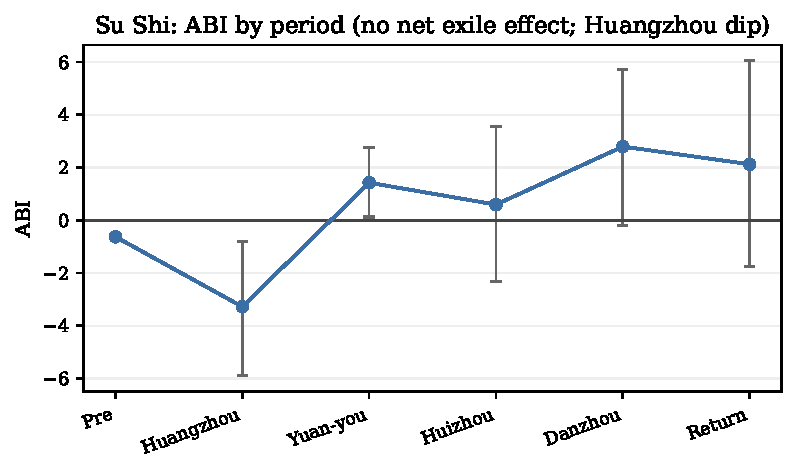
\includegraphics[width=0.62\linewidth]{figures/fig_sushi_period.pdf}
\caption{Su Shi ABI across six periods with 95\% CI. The single dark stretch is Huangzhou ($-3.28$); the net exile effect is not significant (ABI $-0.26$ in vs.\ $+0.31$ outside exile, $p{=}0.55$).}
\label{fig:sushi_period}
\end{figure}


\paragraph{Conditional corroboration (Bai Juyi, grade B).} For Bai Juyi---the only
Tang poet with a usable within-author split---exile (59 poems, Jiangzhou/Zhongzhou) vs.\ merged non-exile (84) gives $\Delta\mathrm{ABI}{=}{+}4.52$ $[-0.22,9.63]$---positive in direction but not separated from zero (two-sided $p{=}0.066$), so it serves as directional corroboration only.
This must not be read as ``exile cheered him up'': 50 of his 66 pre-exile poems are
New Yuefu satires, a genre that saturates the control with 悲苦 lexicon ($12.1$ vs.\
$11.2$ per 1{,}000 characters in exile), so the contrast is confounded by genre selection. The safe claims
are dimensional only: in exile, 贬谪羁旅 self-naming ($+3.66$ $[0.83,6.54]$) and
自然山水 ($+24.3$ $[17.1,32.5]$, the Jiangzhou landscape mode) rise. Accordingly, no pre/post split and no dose gradient are computed for Bai.

\paragraph{Why the remaining four officials are excluded.} 柳宗元 has no usable pre-exile corpus
(fewer than 20 securely datable pre-exile poems); 黄庭坚 has only 4 securely
attached poems; 欧阳修 (12 exile poems) and 王禹偁
(29) fall below pairing power. The within-author claim of this paper therefore
rests on one grade-A analysis, one conditional grade-B check, and four officials
whose data do not support analysis; the claim is scoped accordingly.

\subsection{Transmission robustness}
\label{sec:robust}

A poet's measured profile is a function of the edition in which it is read. We
separate two transmission channels---\emph{reprinting}, in which a shared work
differs only by scribal variation, and \emph{selection}, in which an anthology admits
a subset of the complete collection---and ask what each does to the index.

\paragraph{Reprinting leaves the index intact.} On the Tang side the two sources are
two digitizations of the same complete collection. Across all 432 shared authors the
concordance is $A{=}0.960$ with every dimension preserved ($S{=}5/5$; per-dimension
$r$ from $0.95$ to $0.98$), and no author's sign flips (Figure~\ref{fig:abi}, left;
Table~\ref{tab:tang}). The largest displacement is 柳宗元's ($+0.22\to+0.92$): for an
author whose two affective poles are nearly balanced, the edition moves the
\emph{level} of a near-zero difference without reversing it. A near-perfect profile
agreement ($r{=}0.997$ over the $20$ poet$\times$dimension cells) therefore guarantees
shape and ordering, not the absolute value of a near-zero index.

\begin{table}[H]
\centering\footnotesize
\caption{Tang cross-edition: QTS vs.\ YD (899 \emph{juan}). $\Delta{=}|$ABI
difference$|$. Mean $|\Delta|{=}0.432$; category corr $r{=}0.997$ (20 cells).}
\label{tab:tang}
\begin{tabular}{lrrr}
\toprule
Poet & QTS & YD & $\Delta$\\
\midrule
柳宗元 Liu Zongyuan & $+0.221$ & $+0.922$ & $0.701$\\
刘禹锡 Liu Yuxi & $-0.881$ & $-1.711$ & $0.830$\\
韩愈 Han Yu & $-2.491$ & $-2.587$ & $0.096$\\
白居易 Bai Juyi & $+1.762$ & $+1.863$ & $0.101$\\
\bottomrule
\end{tabular}
\end{table}

\paragraph{Selection moves the dimensions, not the net.} On the Song side we compare
the complete collection against an independently compiled selection anthology,
\emph{Yu Xuan Song Shi}. Across the 253 shared authors ($\ge300$ characters each) the
concordance falls to $A{=}0.557$ (hand lexicon) / $0.567$ (corpus-induced), a moderate
but clearly positive agreement in which three of five dimensions survive at
$|r|\ge0.5$ (Table~\ref{tab:songpop}); the boundary attenuates the author-level signal
without erasing it. An empirical-Bayes hierarchical model on the same authors locates
the effect precisely: the net edition effect is $\hat\delta{=}+0.15$ (95\% CI
$[-0.31,0.59]$), which \emph{contains zero}. The anthology nonetheless carries a
coherent editorial signature (Table~\ref{tab:hb}): it raises nature--landscape by
$+16.68$ per 1{,}000 characters, with easeful ($+1.67$), sorrow--loneliness ($+1.39$)
and void--temporality ($+1.84$) all rising (four CIs excluding zero), while
exile--journey is invariant ($+0.05$). Because the index is a \emph{difference} of two
pole rates, the two poles rise by nearly the same amount and cancel in the net scalar
while remaining visible in the dimensions. Net invariance is a cancellation, not the
absence of an effect.

\begin{table}[H]
\centering\footnotesize
\caption{Song cross-edition at population scale: QSS vs.\ \emph{Yu Xuan Song Shi},
253 shared authors ($\ge$300 chars each). Per-dimension Pearson $r$ of per-1k
rates; values are hand lexicon / corpus-induced lexicon. Dimensions with
$|r|{\ge}0.5$ (preserved) are marked~$^*$.}
\label{tab:songpop}
\begin{tabular}{lcc}
\toprule
Dimension & M1 $r$ & Induced $r$\\
\midrule
悲苦孤寂 Bei & $0.55^*$ & $0.59^*$\\
贬谪羁旅 Bian & $0.45$ & $0.41$\\
旷达闲适 Kuang & $0.47$ & $0.40$\\
自然山水 Zi & $0.69^*$ & $0.63^*$\\
空幻时空 Kong & $0.60^*$ & $0.61^*$\\
\bottomrule
\end{tabular}
\end{table}
\begin{table}[H]
\centering\footnotesize
\caption{Empirical-Bayes hierarchical noise floor (Song side, 253 shared authors).
The edition effect $\delta$ is the inverse-variance-weighted difference between
anthology and complete-collection ABI; its 95\% CI includes $0$
$\Rightarrow$ net-index invariance. The per-dimension $\delta_d$ (per 1{,}000
characters) exposes the anthology's editorial signature; $^*$ marks a 95\% CI
excluding $0$.}
\label{tab:hb}
\begin{tabular}{lcc}
\toprule
Quantity & Estimate & 95\% CI\\
\midrule
Edition effect $\delta$ (net index) & $+0.15$ & $[-0.31,\,0.59]$\\
Latent mean $\mu$ & $+0.82$ & $[0.32,\,1.30]$\\
Latent SD $\tau$ & $3.64$ & $[3.24,\,4.01]$\\
\midrule
\multicolumn{3}{l}{\emph{Per-dimension edition effect $\delta_d$ (per 1k chars)}}\\
悲苦孤寂 sorrow & $+1.39^*$ & $[1.08,\,1.70]$\\
贬谪羁旅 exile & $+0.05$ & $[-0.19,\,0.28]$\\
旷达闲适 easeful & $+1.67^*$ & $[1.34,\,2.00]$\\
自然山水 nature & $+16.68^*$ & $[16.06,\,17.29]$\\
空幻时空 void & $+1.84^*$ & $[1.43,\,2.25]$\\
\bottomrule
\end{tabular}
\end{table}

\paragraph{A second anthology replicates the signature.} A signature seen once is an
anecdote. We therefore add \emph{Song Shi Chao} (宋詩鈔, kanripo KR4h0157), a private
Qing anthology, parsed into 9{,}612 poems by 76 authors. All five dimensions shift in
the \emph{same direction} in both anthologies (signs agree $5/5$) and the two effect
vectors correlate at Pearson $0.95$ (Table~\ref{tab:rep}); the correlation is driven
by the nature--landscape shift, which dominates both (official $+16.7$, private
$+4.4$ per 1{,}000 characters). Directional predictions registered pre-hoc from the
two anthologies' documented selection principles hold for the imagery registers and
fail for the easeful one---both raise 旷达闲适---so the signature is
\emph{lexicon-conditional}. What replicates is the \emph{shape} of editorial
intervention and its concentration in the imagery registers, not its magnitude, and
it converges at the group level: over the 68 authors common to all three sources the
per-author shifts correlate at only $r{=}-0.11$ to $0.40$. Net invariance, moreover,
belongs to the imperial anthology alone; \emph{Song Shi Chao} moves the net quantity
clear of zero ($\hat\delta{=}-0.69$, 95\% CI $[-1.09,-0.28]$). The dimension-level
signature generalises across anthologies; the invariance of the net scalar does not.

\begin{table}[H]
\centering\footnotesize
\caption{The editorial signature in two independently compiled Song selection
anthologies. $\delta_d$ = inverse-variance-weighted edition effect (anthology minus
complete collection, per 1{,}000 characters); $^*$ = 95\% CI excluding $0$. Signs
agree on 5/5 dimensions (with $n{=}5$ we cannot test significance; we report both
5/5 and 4/5 agreement); the $\delta$ vectors correlate at Pearson $0.95$. The
right-hand column gives the direction registered pre-hoc from the anthologies'
documented selection principles, before the second anthology was read.}
\label{tab:rep}
\begin{tabular}{lccc}
\toprule
Dimension & \emph{Yu Xuan Song Shi} & \emph{Song Shi Chao} & Registered (pre-hoc)\\
\midrule
悲苦孤寂 sorrow & $+1.39^*$ & $+1.53^*$ & up---held\\
贬谪羁旅 exile & $+0.05$ & $+0.15$ & up---held (small magnitude)\\
旷达闲适 easeful & $+1.67^*$ & $+0.88^*$ & near zero---not held\\
自然山水 nature & $+16.68^*$ & $+4.43^*$ & up, less than imperial---held\\
空幻时空 void & $+1.84^*$ & $+0.03$ & indeterminate\\
\bottomrule
\end{tabular}
\end{table}

\paragraph{Discord lives in the set of works, not the text.} The coefficients above
pool all the text an author has in a source and so assume the two channels carry
comparable sets of works. Keying every work on (author, title) and re-flowing each
witness onto a common work boundary separates the two mechanisms
(Table~\ref{tab:realign}). On the Tang side $93.3\%$ of characters already fall on
shared works and realignment barely moves the reading ($0.960\to0.966$). The three
Song pairings share only $7.5\%$, $21.6\%$ and $14.2\%$ of their characters---an
anthology simply holds a different set of poems---yet once only works present in both
sources are compared, concordance rises uniformly to $0.90$--$0.96$. Alignment does
not achieve this by collapsing the strings: of the works QSS shares with the two
anthologies, none is byte-identical and mean character similarity is only
$0.80$/$0.84$. Cross-edition discord is concentrated at the level of the \emph{set of
works}, not the \emph{text}---a descriptive characterisation, not a causal claim that
the text layer is edition-independent. Table~\ref{tab:invariance} collects the
concordances and Figure~\ref{fig:abi} the author-level scatter; a clustered-author
bootstrap ($B{=}2000$) attaches a 95\% CI to each headline coefficient.

\begin{table}[H]
\centering\footnotesize
\caption{Work-level realignment. \emph{Pooled} = all text the author has in that
source (the basis of the tables above); \emph{Aligned} = only works present in both
sources (key as defined in text). Coverage = matched-work characters divided by
pooled characters. 95\% CI from a clustered-author bootstrap ($B{=}2000$ author-level resamples); $n$ = authors in the pooled / aligned estimate.}
\label{tab:realign}
\begin{tabular}{lcccr}
\toprule
Pair & $A$ pooled (95\% CI) & $A$ aligned (95\% CI) & $n$ (pool/align) & Coverage\\
\midrule
Tang: QTS vs.\ YD (two digitizations, same work) & $0.960\,[0.948,0.971]$ & $0.966\,[0.957,0.974]$ & $432/415$ & $0.932$\\
Song: QSS vs.\ \emph{Yu Xuan Song Shi} & $0.557\,[0.459,0.647]$ & $0.899\,[0.853,0.936]$ & $253/179$ & $0.075$\\
Song: QSS vs.\ \emph{Song Shi Chao} & $0.822\,[0.630,0.921]$ & $0.957\,[0.924,0.979]$ & $75/73$ & $0.216$\\
Song: \emph{Yu Xuan} vs.\ \emph{Song Shi Chao} & $0.634\,[0.460,0.768]$ & $0.961\,[0.896,0.987]$ & $68/51$ & $0.142$\\
\bottomrule
\end{tabular}
\end{table}
\begin{table}[H]
\centering\footnotesize
\caption{Cross-edition concordance across the source pairings. $A$ = concordance
(Pearson $r$ of net ABI); $S$ = structural concordance (fraction of 5 dimensions
with $|r|{\ge}0.5$). All pairs use authors with $\ge$300 characters in both sources;
the last two rows further restrict to the 68 authors present in all three Song
sources, making the two anthologies comparable. Bootstrap 95\% CIs for the headline pooled coefficients are $[0.948,0.971]$ (Tang), $[0.459,0.647]$ (QSS/Yu Xuan), and $[0.630,0.921]$ (QSS/Song Shi Chao); each is significantly above zero.}
\label{tab:invariance}
\begin{tabular}{lcccr}
\toprule
Comparison & Lexicon & $n$ & $A$ & $S$\\
\midrule
Tang: QTS vs.\ YD (same work) & M1 & 432 & $0.960$ & $5/5$\\
Tang: QTS vs.\ YD (same work) & induced & 432 & $0.938$ & $5/5$\\
Song: QSS vs.\ Yu Xuan (selection) & M1 & 253 & $0.557$ & $3/5$\\
Song: QSS vs.\ Yu Xuan (selection) & induced & 253 & $0.567$ & $3/5$\\
Song: QSS vs.\ Song Shi Chao (selection) & M1 & 75 & $0.822$ & $5/5$\\
Song: QSS vs.\ Yu Xuan, matched authors & M1 & 68 & $0.601$ & $4/5$\\
Song: QSS vs.\ Song Shi Chao, matched authors & M1 & 72 & $0.827$ & $5/5$\\
\bottomrule
\end{tabular}
\end{table}
\begin{figure}[t]
\centering
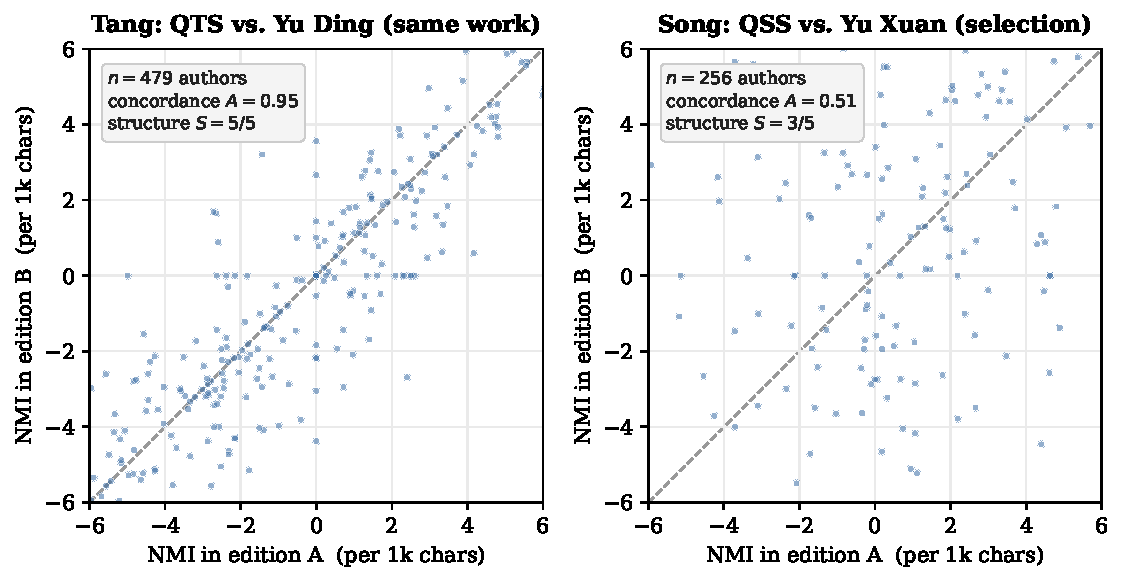
\includegraphics[width=0.84\linewidth]{figures/abi_cross_edition.pdf}
\caption{The transmission-robustness control, one point per shared author (ABI
in edition A vs.\ edition B; dashed line is perfect agreement).
\textbf{Left:} Tang, \emph{Quan Tang Shi} vs.\ \emph{Yu Ding Quan Tang Shi}---two
digitizations of the \emph{same} work; 432 authors lie tightly along the diagonal
($A{=}0.960$, $S{=}5/5$).
\textbf{Right:} Song, \emph{Quan Song Shi} vs.\ the imperial \emph{Yu Xuan Song Shi}
\emph{selection anthology}---a \emph{different} work; 253 authors form a visibly
looser cloud ($A{=}0.557$, $S{=}3/5$). The anthology shifts individual scores without
a systematic net shift (Tables~\ref{tab:hb} and~\ref{tab:rep}), which is why the
cloud loosens but does not drift. The second Song anthology is reported numerically
in Table~\ref{tab:rep}.}
\label{fig:abi}
\end{figure}

\paragraph{Counterfactual channels.} Projecting each author's posterior dimension
rates through each channel quantifies how much of a profile is the survivor's. At the
aggregate level every channel shift is small next to the author-population
heterogeneity ($\tau\approx3.6$): $+0.15$ (official), $-0.68$ (private) and $-0.04$
(Tang reprint). The five-dimensional profile is another matter
(Figure~\ref{fig:counterfactual_delta}): both anthologies inflate every dimension in
the same direction, nature--landscape dominating, so the net effect is small only
because the poles cancel. At the author level the asymmetry becomes concrete: 陆游
($+0.57$), 苏轼 ($+0.41$) and 欧阳修 ($-0.18$) all change sign under the private
channel, whereas 秦观's bleakness ($-2.11$ / $-1.56$ / $-2.72$) and 王禹偁's
near-neutrality survive every channel. Across the 256 Song authors the ranking is
globally stable (Spearman $0.96$ between corpus and official-channel ABI), but
$13.6\%$ of pairwise orders change and 26 authors shift with a CI excluding zero,
against a null expectation of $\approx13$. The Tang reprint channel, by contrast,
displaces authors in common mode without reshuffling them: 刘禹锡's counterfactual
($-1.26$) lies between his two edition-level measurements ($-0.88$, $-1.71$).
Author-level \emph{reshaping} is a property of selection; for the Song poets the
transmission channel is a visible, dimension-specific co-author of the measured
profile.

\begin{figure}[t]
\centering
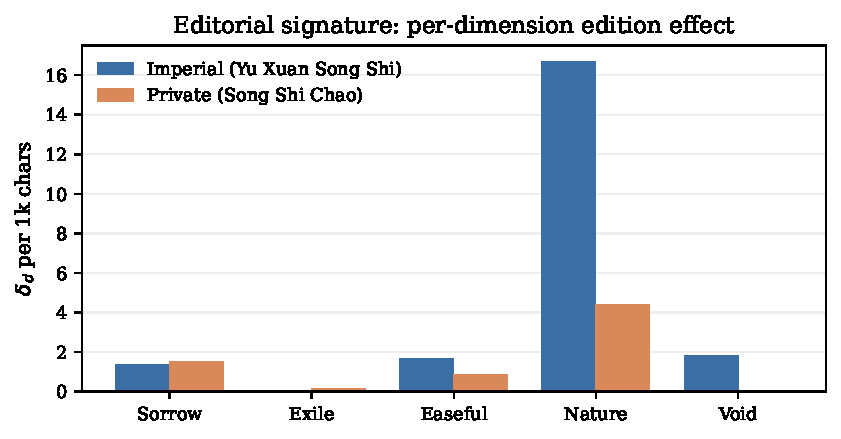
\includegraphics[width=0.62\linewidth]{figures/fig_counterfactual_delta.pdf}
\caption{Both anthologies shift all five dimensions in the same direction; nature--landscape dominates (imperial $+16.7$, private $+4.4$ per 1k).}
\label{fig:counterfactual_delta}
\end{figure}

\section*{Limitations}
\begin{itemize}
\item (a) The author-level criterion $r{=}0.57$ validates the short-poem gold
  subsample, not the full-collection values in Table~\ref{tab:abi}.
\item (b) The CNN recovers only the two emotional poles (sorrow--loneliness,
  detached--easeful); the three middle dimensions stay flat at zero in prediction.
\item (c) 26 of 256 authors have CIs crossing zero, against a global null
  expectation of $\approx$13.
\item (d) Small-corpus authors such as 辛弃疾 are version-uncontrolled, so their
  placements rest on the corpus alone.
\end{itemize}

\section{Conclusion}
\label{sec:conclusion}

We have presented a reproducible instrument for the affective measurement of
Tang--Song exile poetry and used it to place twelve named banished officials on a
single scale. The instrument is a character-level CNN that predicts a transparent
five-dimensional lexicon's scalar index directly from raw characters
($r{=}0.934$); its profiles separate the bleak (韩愈, 秦观) from the clearly easeful
(白居易, 黄庭坚, 范仲淹, 辛弃疾) and leave the remaining five indistinguishable from
neutral. A lexicon-perturbation check sharpens the distinction: the six near-zero
placements carry sign-flip rates above $20\%$ and are read as conditional on the full
lexicon, while the six clearly polarised placements hold their sign in at least
$90\%$ of draws (Table~\ref{tab:abi}). Because the network is trained on the lexicon,
its agreement with blind human coding ($\rho{=}0.46$ poem-level, $r{=}0.57$
author-level) bounds the lexicon's validity rather than checking it independently,
and the index is loaded unevenly across dimensions---the easeful pole that defines it
remains the weakest ($0.29$). Five categories cannot carry irony or
allusion-dependent affect; the three registers recovered from the analyser's
residuals (quietism, homesickness, travel-and-duty) were blind-verified and merged
into the lexicon (Supplementary Material, App.~C).

The second contribution is measurement-theoretic. A poet's score is a function of
the edition in which it is read. Two digitizations of one Tang work leave the index
essentially unchanged ($A{=}0.960$), but two independently compiled Song anthologies
raise imagery and easeful vocabulary in a consistent, dimension-level pattern: the
net scalar survives the imperial anthology and shifts under the private one.
Cross-edition discord is concentrated in the \emph{set of works} a compiler chose,
not in the text of any single poem, so an affect score reported from a single edition
is in part an editorial decision. The same framework supplies a counterfactual
projection that attributes a measured profile to its transmission channels, and a
within-author analysis of 苏轼 that finds no net exile effect but a brightening
lexical profile with severity---three periods only, and offered as a directional
observation alongside the exile-gloom scholarship rather than as its refutation.

The instrument's limits are measured rather than assumed: the gold standard is small
and drawn from the same corpus family as the lexicon, the selection test covers only
two Song anthologies of \emph{Siku} ancestry, and the corpus is restricted to
\emph{shi} verse.


All texts are public-domain classical works; no personal or non-public data are
used. The two blind coders who produced the human gold standard provided informed
consent and were compensated for their work; no personal data about them are
released, and their dual-coded annotations are published only as de-identified
text. Quantitative scores are intended to complement, not replace, humanistic close
reading.

\section*{Data and Code Availability}
\label{sec:repro}
All sources are public-domain classical works. Corpora: \emph{Quan Tang Shi} and
\emph{Quan Song Shi} (Book1Q84 / Chinese Textware digital editions, 2025 snapshot) and
two kanripo transcriptions of Kangxi- and Qing-era anthologies (KR4h0143 of the
\emph{Song Jin Yuan Ming Si Chao Shi} \citep{kangxi1709}; KR4h0157 of \emph{Song Shi
Chao} \citep{wu1671}), both in the \emph{Siku Quanshu} Wenyuange base edition; edition
and snapshot identifiers are recorded in the companion repository. The measuring
instrument, the supplement, and every analysis script are openly available at
\url{https://github.com/fourhairsall/tangsong-exile-affect}, together with the
de-identified dual codings (\texttt{annotations/}) and the orchestrator
\texttt{recompute\_all.py} that regenerates every number from the raw corpora and
writes \texttt{numbers\_ledger.json}, mapping each reported quantity to its source
script and result key. Every stochastic step pins a fixed seed (NumPy,
\texttt{random}, \texttt{torch.manual\_seed}); the manuscript is compiled with
\texttt{xelatex} for the CJK glyphs. All deep-learning experiments ran on a single
workstation (CPU training, PyTorch~2.14.0+\texttt{cpu}; Chinese text normalised with
OpenCC), with exact package pins in \texttt{requirements.txt}.

\bibliographystyle{plainnat}
\begin{thebibliography}{9}
\bibitem[Kim(2014)]{kim2014convolutional}
Y.~Kim.
\newblock Convolutional neural networks for sentence classification.
\newblock In \emph{EMNLP}, 2014.

\bibitem[Stamatatos(2009)]{stamatatos2009survey}
E.~Stamatatos.
\newblock A survey of modern authorship attribution methods.
\newblock \emph{Journal of the American Society for Information Science
and Technology}, 60(3):538--556, 2009.

\bibitem[Hou and Frank(2015)]{hou2015sentiment}
Y.~Hou and A.~Frank.
\newblock Analyzing sentiment in classical Chinese poetry.
\newblock In \emph{Proc.\ of the 3rd Workshop on Language Technology for
Cultural Heritage, Social Sciences, and Humanities (LaTeCH)}, 2015.

\bibitem[Du et al.(2025)]{du2025multimodal}
X.~Du, H.~Pei, and H.~Zhang.
\newblock Picturized and Recited with Dialects: A Multimodal Chinese
Representation Framework for Sentiment Analysis of Classical Chinese
Poetry.
\newblock \emph{arXiv preprint arXiv:2505.13210}, 2025.

\bibitem[Liu and Zhao(2025)]{liu2025samcap}
Z.~Liu and W.~Zhao.
\newblock Sentiment analysis of Chinese ancient poetry based on multidimensional
attention under the background of digital intelligence integration.
\newblock \emph{Libri}, 75(1):97--108, 2025. DOI: 10.1515/libri-2024-0053.

\bibitem[Qin et al.(2025)]{qin2025shades}
Z.~Qin, S.~Ng, and Y.~Song.
\newblock Shades of grey: Quantifying a database of 18 aesthetic moods in
classical Chinese poetry.
\newblock \emph{Empirical Studies of the Arts}, 43(2):1181--1213, 2025.
DOI: 10.1177/02762374241305561.

\bibitem[Zhou et al.(2022)]{shiziren2022}
A.~Zhou, C.~Sang, Y.~Zhang, and M.~Lu.
\newblock 诗人密码: 唐诗作者身份识别 (The Poet Code: Tang Poetry Authorship
Identification).
\newblock \emph{Journal of Chinese Information Processing
(中文信息学报)}, 36(6):162--170, 2022. DOI: 10.3969/j.issn.1003-0077.2022.06.017.

\bibitem[Zhou et al.(2021)]{zhou2021lda}
A.~Zhou, Y.~Zhang, H.~Wei, and M.~Lu.
\newblock LDA-Transformer Model in Chinese Poetry Authorship Attribution.
\newblock In \emph{Information Retrieval: 27th China Conference, CCIR 2021,
Dalian, China, October 29--31, 2021, Proceedings (LNCS, vol.~13026)}, pages
59--73. Springer, 2021. DOI: 10.1007/978-3-030-88189-4\_5.

\bibitem[Fang(2011)]{fang2011cld}
A.~C.~Fang, W.-y.~Li, and J.~Cao.
\newblock In search of poetic discourse of classical Chinese poetry: an
  imagery-based stylistic analysis of Liu Yong and Su Shi.
\newblock \emph{Chinese Language and Discourse}, 2(2):232--249, 2011.
  John Benjamins. DOI: 10.1075/cld.2.2.04fan.

\bibitem[Yuan et al.(2023)]{yuan2023variants}
L.~Yuan, D.~Wang, and S.~Huang.
\newblock Automatic discovery of parallel textual variants in classical
Chinese texts.
\newblock \emph{Journal of Library Science in China (图书情报工作)} /
ChinaXiv: chinaxiv-202304.00607, 2023.

\bibitem[Song et al.(2022)]{bianzhe2022}
X.~Song, X.~Huo, Y.~Liu, and J.~Deng.
\newblock 数字人文视角下《全唐诗》贬谪诗人的时空轨迹分析 (Spatiotemporal
Trajectory of Exiled Poets in the Complete Tang Poems).
\newblock \emph{Library and Information Service (图书情报工作)}, 66(7):26--34,
2022. DOI: 10.13266/j.issn.0252-3116.2022.07.003.

\bibitem[Wang and Zhu(2023)]{wang2023lideyu}
Q.~Wang and T.~Zhu.
\newblock Use data for education: Li Deyu's self-reported texts of two
demotions as an example.
\newblock In \emph{Proc.\ of ICAIE}, Atlantis Press, 2023.
DOI: 10.2991/978-94-6463-242-2\_36.

\bibitem[Wang and Sun(2008)]{wang2008finding}
王兆鹏, 孙凯云.
\newblock 寻找经典——唐诗百首名篇的定量分析.
\newblock 《文学遗产》, 2008(2):40--52.

\bibitem[Shang(2007)]{shang2007exiled}
尚永亮.
\newblock 《唐五代逐臣与贬谪文学研究》.
\newblock 武汉大学出版社, 2007.

\bibitem[Xing(2024)]{xing2024liusu}
邢若琳.
\newblock 论柳宗元、苏轼流寓心态之异同.
\newblock 《今古文创》, 2024(36):52--55.

\bibitem[Kangxi(1709)]{kangxi1709}
康熙 (Kangxi Emperor), 御定.
\newblock 御選宋金元明四朝詩 (Yu Xuan Song Jin Yuan Ming Si Chao Shi).
\newblock Imperial anthology, 1709. Transcription: kanripo KR4h0143
(\emph{Siku Quanshu} base edition).

\bibitem[Wu(1671)]{wu1671}
吳之振 (Wu Zhizhen), 編.
\newblock 宋詩鈔 (Song Shi Chao).
\newblock Private anthology, Qing dynasty; \emph{Siku Quanshu} Wenyuange text,
106 \emph{juan}. Transcription: kanripo KR4h0157 (\emph{Siku Quanshu} base
edition).

\bibitem[Lou and Yu(2025)]{overlock2025}
M.~Lou and Y.~Yu.
\newblock OverLoCK: An Overview-first-Look-Closely-next ConvNet with
Context-Mixing Dynamic Kernels.
\newblock In \emph{Proc.\ of the IEEE/CVF Conference on Computer Vision and
Pattern Recognition (CVPR)}, 2025 (Oral). arXiv:2502.20087.

\bibitem[Lou et al.(2025)]{transxnet2025}
M.~Lou, S.~Zhang, H.-Y.~Zhou, S.~Yang, C.~Wu, and Y.~Yu.
\newblock TransXNet: Learning Both Global and Local Dynamics with a Dual Dynamic
Token Mixer for Visual Recognition.
\newblock \emph{IEEE Transactions on Neural Networks and Learning Systems
(TNNLS)}, 2025. arXiv:2310.19380.

\bibitem[Cai et al.(2026)]{pfgn2026}
X.~Cai, C.~Sun, Y.~Wang, H.~Yang, and Y.~Wu.
\newblock PFGNet: A Fully Convolutional Frequency-Guided Peripheral Gating
Network for Efficient Spatiotemporal Predictive Learning.
\newblock In \emph{Proc.\ of CVPR}, 2026. arXiv:2602.20537.

\bibitem[Hsing and Tu(2026)]{tacnn2026}
C.-W.~Hsing and W.-L.~Tu.
\newblock Tensor-Augmented Convolutional Neural Networks: Enhancing Expressivity
with Generic Tensor Kernels.
\newblock \emph{arXiv preprint arXiv:2604.08072}, 2026.

\bibitem[Farvardin and Chapman(2026)]{facnn2026}
P.~Farvardin and D.~Chapman.
\newblock End-to-end Feature Alignment: A Simple CNN with Intrinsic Class
Attribution.
\newblock \emph{arXiv preprint arXiv:2603.25798}, 2026.

\end{thebibliography}

\end{document}
